%% This is an example first chapter.  You should put chapter/appendix that you
%% write into a separate file, and add a line \include{yourfilename} to
%% main.tex, where `yourfilename.tex' is the name of the chapter/appendix file.
%% You can process specific files by typing their names in at the 
%% \files=
%% prompt when you run the file main.tex through LaTeX.
\chapter{Webauthn Firewall Design}\label{Chap:WebauthnFirewallDesign}

This chapter describes the high-level design of the webauthn firewall and how it fits within an existing web-application. It also describes how a software engineer would use the different configuration options and tools that the firewall provides in order to secure a web-service.

\subsection{Overview}

The webauthn firewall acts as a Web Application Firewall (WAF). It is situated directly between the frontend and backend, processing all user requests sent between the two. Its main purpose is to simplify integrating webauthn transaction authentication into a web-service. Traditional methods of directly integrating webauthn into a web-service is bulky and difficult to configure. The firewall is designed to be highly configurable and minimally intrusive. The less code an engineer has to modify in the web-service itself, the better.

The overall function of the firewall is to capture and parse HTTP requests between the frontend and backend. Then it must decide whether to verify those requests with transaction authentication or not. If not, the request is simply proxied through to the backend without any extra work. Otherwise, performs a verification procedure on the request and only upon success does the request pass through the firewall to the backend. Upon failure, the request is blocked.

\begin{center}
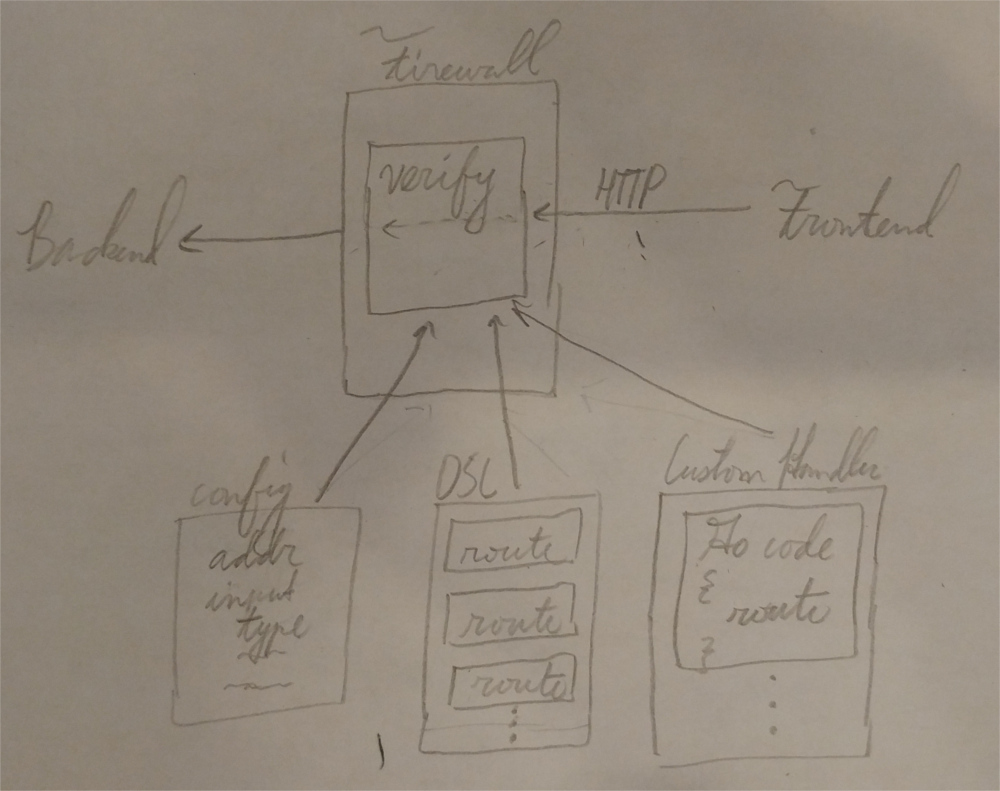
\includegraphics[width=12cm]{firewall_configuration}
\end{center}

A number of components come together in the firewall to enable its function. There is a central configuration element for the whole firewall. A number of core webauthn routes are protected automatically. But the rest of the application specific routes are configured using a domain specific language or custom Go code. Configurations can be easily modified and completely define how the firewall webauthn secures a web-service.

Apart from configuration ease, the design of a webauthn firewall is very powerful because it is minimally intrusive, almost transparent to the web-service it is securing. The backend is completely unaware that the requests it receives are webauthn authenticated. The frontend has to interface with the user's hardware authenticator device, so it must be aware of webauthn, but only to a minor extent. As a result, deployment of the webauthn firewall is simple and seamless.

%% 
%% \iffalse
%% it needs transaction authentication, the firewall acts as a gatekeeper for that request.


%% Each request gets parsed by the firewall, and understood whether it is a request that needs webauthn transaction authentication or not. If not, the request is simply proxied through to the backend without any extra work. However, if it needs transaction authentication, the firewall acts as a gatekeeper for that request. The firewall performs a verification procedure on the request and only upon success does the request pass through the firewall to the backend. If it fails, the firewall returns an error back to the frontend. This design strategy for integrating webauthn transaction authentication into a service is very powerful because it is web service agnostic. The backend is completely unaware that the requests it receives are webauthn authenticated. Of course, since the frontend has to interface with the user's hardware authenticator device, it must be aware of webauthn, but only to a minor extent. 
%% \fi
%% 

\subsection{Proxying Requests}

In three different case studies, the firewall is used to integrate webauthn transaction authentication into two different paradigms of web service designs, RESTful and server-side rendered websites. For each, the notion of the firewall being situated between the frontend and backend is slightly different, but the function and role of the webauthn firewall is the same, filtering, verifying and proxying requests. 

\begin{center}
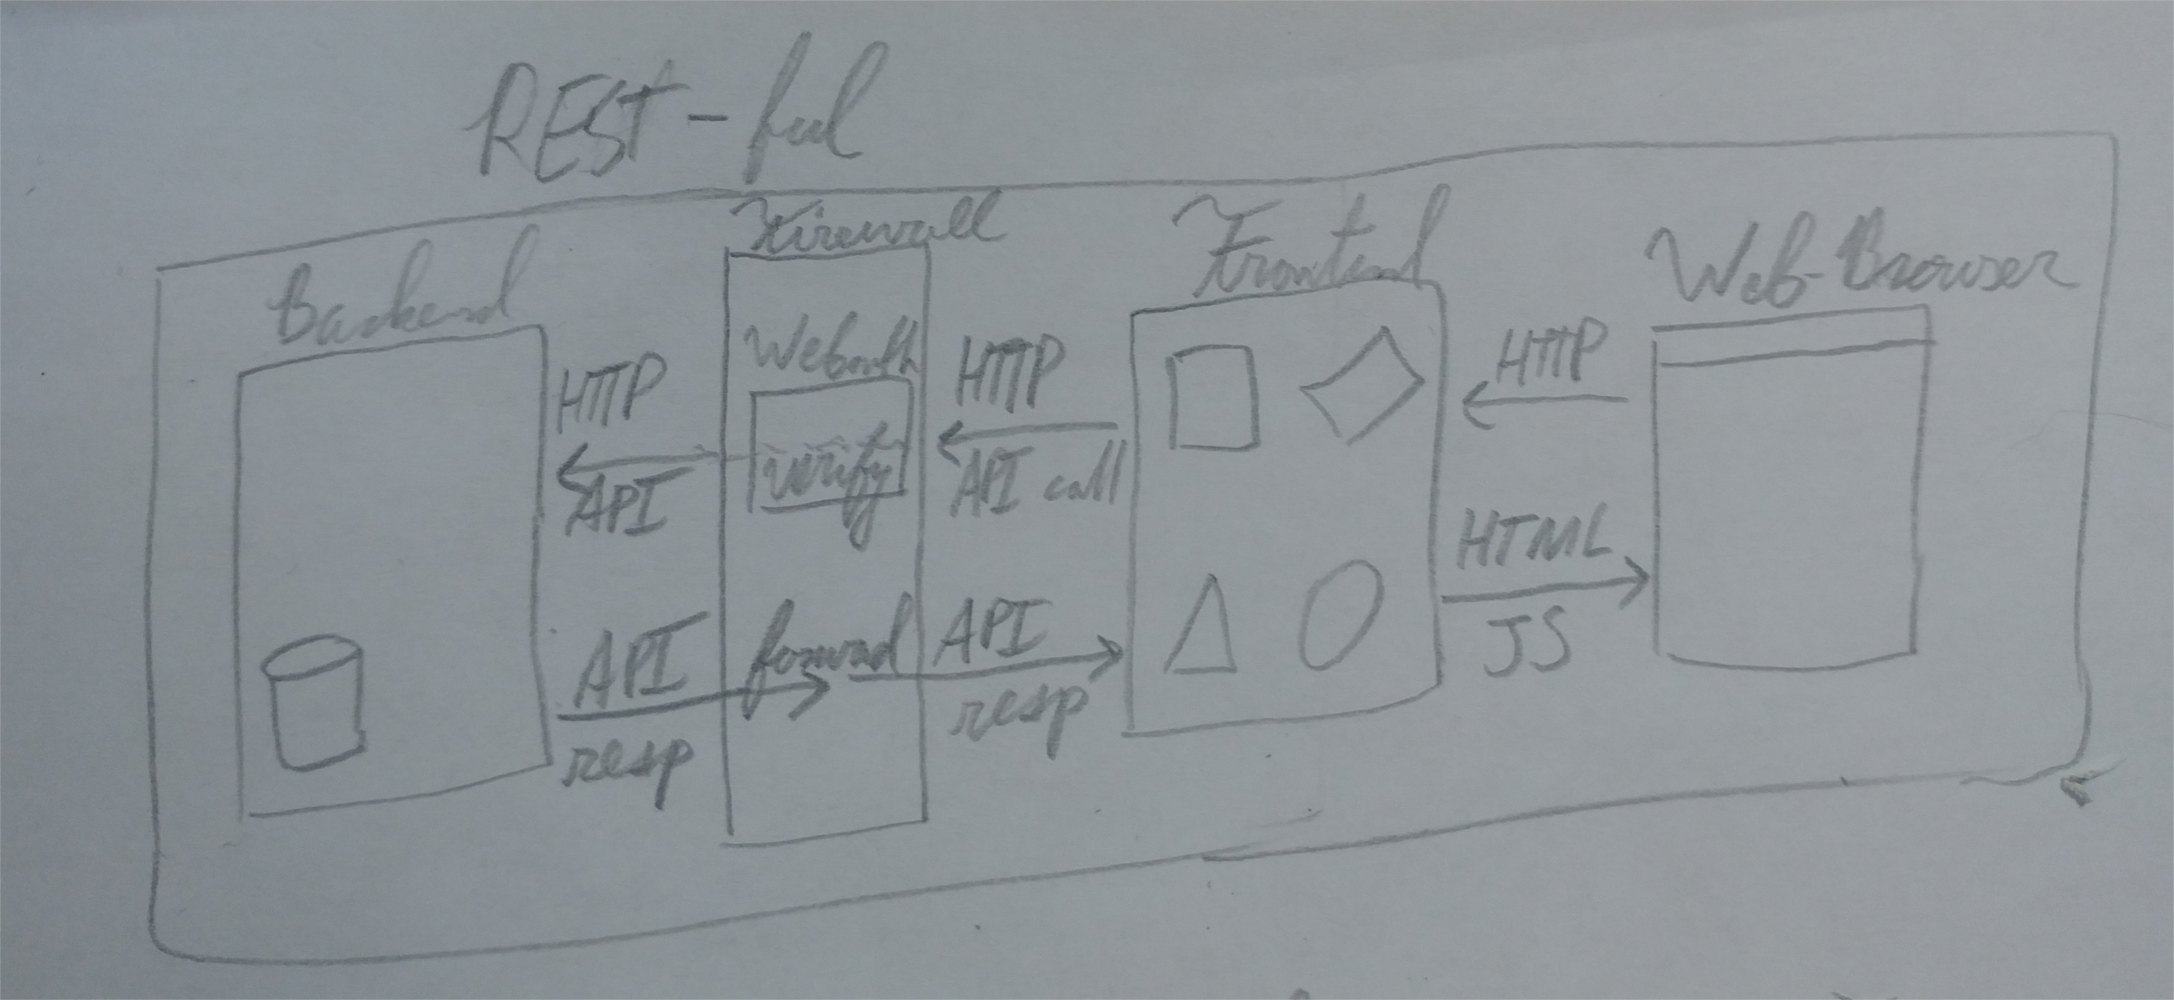
\includegraphics[width=12cm]{restful_with_firewall}
\end{center}

For a RESTful web application, the placement of the firewall is more intuitive. In a RESTful design, frontend and backend are separate programs running on their own IP addresses and ports. The user's web-browser interacts with the frontend through its IP address. And whenever the frontend needs to interact with the backend, it launches HTTP requests to the IP address of the backend. However, the webauthn firewall must sit in between the two. So, the firewall runs on its own IP address and port, and the frontend is reconfigured to use it as its backend address destination. So when the frontend needs to issue a backend request, it sends it rather to firewall rather than the backend. From there, the firewall performs its role and, as necessary, proxies onward to the actual backend. Responses from the backend are returned to the firewall which are automatically forwarded on to the frontend. 

\begin{center}
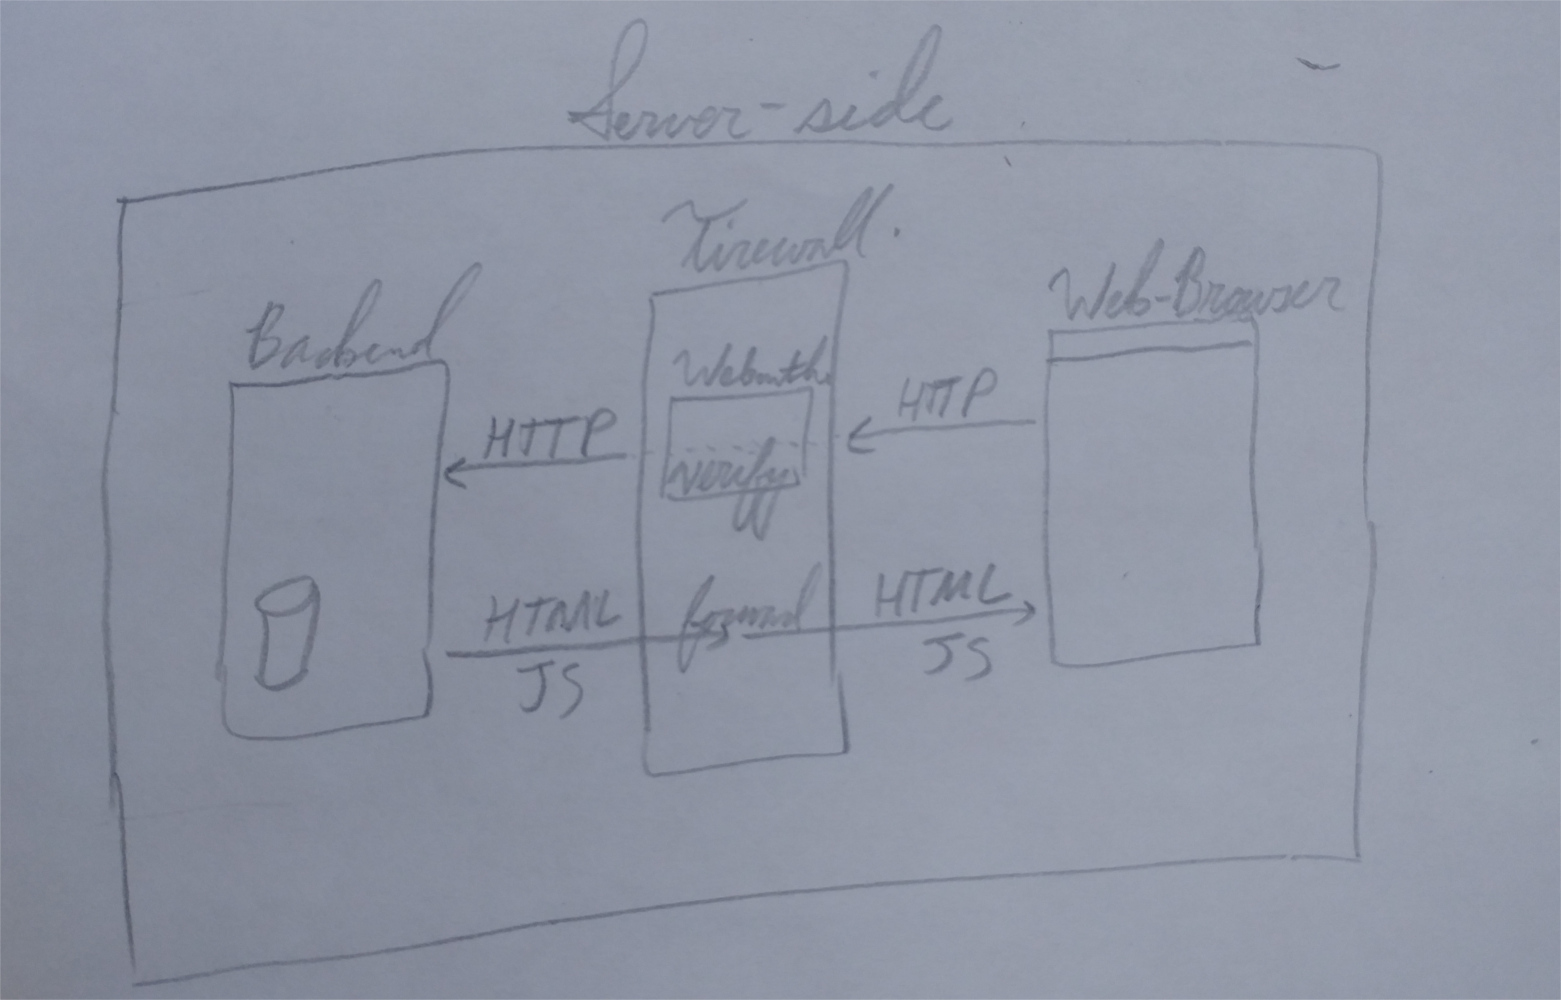
\includegraphics[width=12cm]{serverside_with_firewall}
\end{center}

In a server-side rendering web application, the firewall additionally performs the role of the frontend described in the RESTful use case. That is, the user's web-browser interacts with the IP address of the firewall directly. All HTTP requests originate from the user's web-browser and are directed to whatever the address is of the frontend. In a server-side rendering web application, the whole service, the frontend and backend, is served out of the same address. With the webauthn firewall, requests get sent to the firewall which again does its role and, if necessary, relays onward to the server-side rendering web-application. In this case, the webauthn firewall is situated between the web-browser and backend. But nonetheless, it is the same principle as with the RESTful web application use case. An origin, in this case the web-browser, issues requests destined for a backend, but they get intercepted by the firewall, before they continue on if everything succeeds.

\subsection{Webauthn Firewall Configuration}

%% TODO: Make option in firewall to either pass through or block non-specified requests. Modify this paragraph

As the webauthn firewall filters requests sent to it, some requests will be held back to be webauthn transaction authenticated first. Which requests get held back and what their authentication messages are is configured in the firewall by the software engineer. In order to specify which HTTP route get filtered out and transaction authenticated, the engineer simply includes the route in the firewall's configuration. All other routes not specified in the configuration are simply passed on through to the backend without any checks.

\subsubsection{Configuration Parameters}\label{Sec:ConfigurationParameters}

The webauthn firewall has a number of configurable parameters that aid and dictate how routes get secured. The following is the firewall configuration for Conduit:

\begin{lstlisting}
  firewallConfigs := &wf.WebauthnFirewallConfig{
    RPDisplayName: "Foobar Corp.",
    RPID:          "localhost",

    FrontendAddress:       frontendAddress,
    ReverseProxyTargetMap: reverseProxyTargetMap,
    ReverseProxyAddress:   reverseProxyAddress,

    GetUserID: userIDFromJWT,
    ContextGetters: wf.ContextGettersType{
      "comment":      commentFromCommentID,
      "article":      articleFromArticleSlug,
      "current_user": getCurrentUser,
    },

    WebauthnCorePrefix: "/api/webauthn",
    LoginURL:           "/api/users/login",
    LoginGetUsername: func(r *wf.ExtendedRequest) (string, error) {
      return r.Get_WithErr("user", "username")
    },

    SupplyOptions: true,
    Verbose:       true,
  }
\end{lstlisting}

The fields within the configuration are grouped by function. The first group, \lstinline{RPDisplayName} and \lstinline{RPID}, is used by the webauthn library when setting up and verifying transaction authentication events. 

\begin{center}
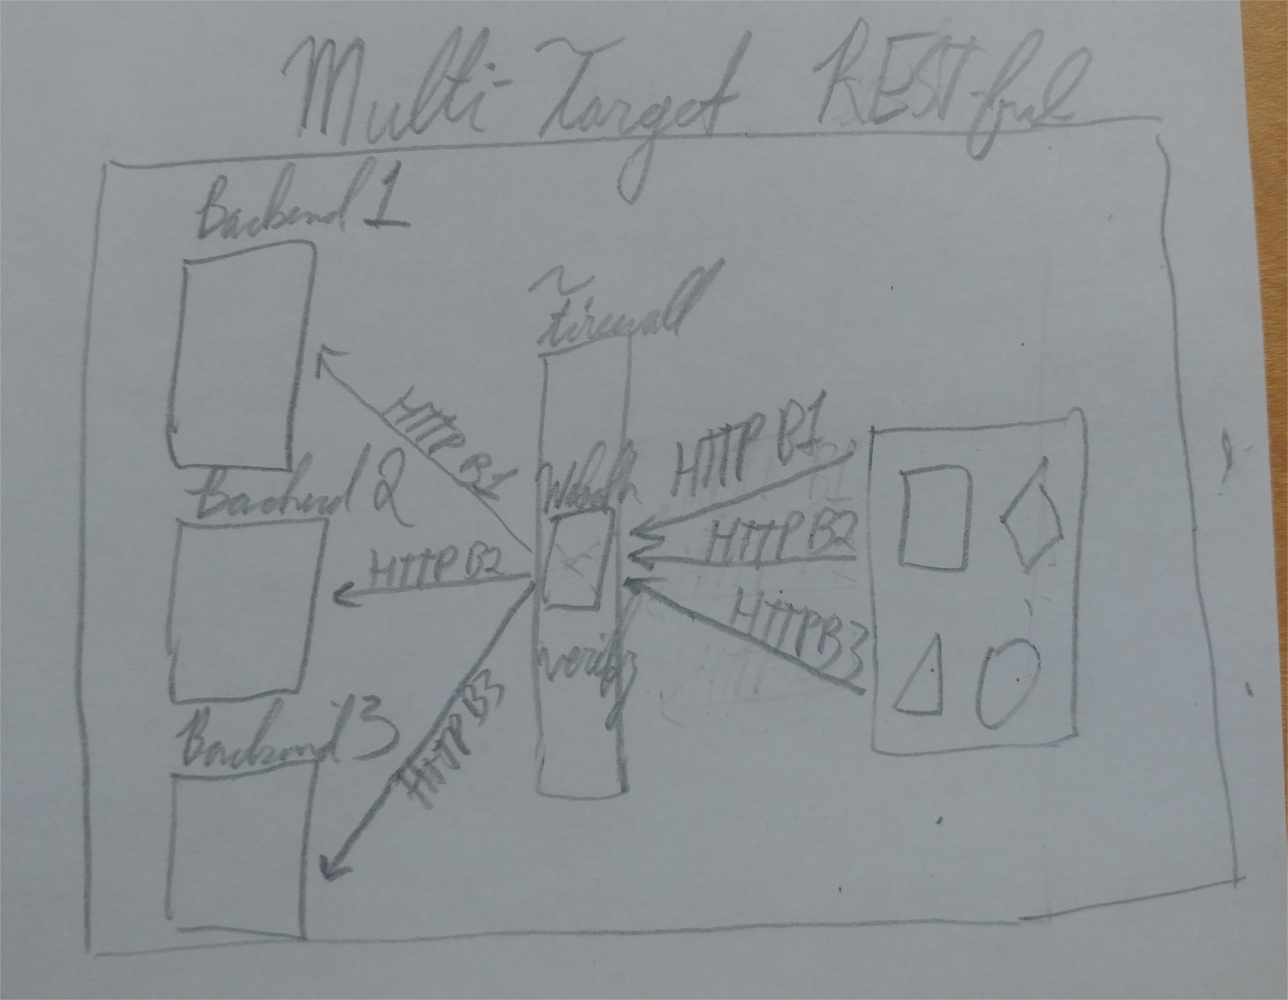
\includegraphics[width=12cm]{multitarget_restful}
\end{center}

The second group, \lstinline{FrontendAddress}, \lstinline{ReverseProxyTargetMap} and \lstinline{ReverseProxyAddress}, contains the proxying address information. They hold the address of the frontend, the target backends and the firewall itself, respectively. It is possible that a web-service's frontend accesses multiple backends. In which case, the firewall has to know which backend gets forwarded incoming requests after processing them. This is stored as a hash map of hosts and target backends in \lstinline{ReverseProxyTargetMap}. This field simply configures the firewall to catch requests of a given \lstinline{host} address and forward it to a specific \lstinline{target}.

%% 
%% \iffalse
%% \begin{itemize}[nosep]
%% \item \lstinline{FrontendAddress}: Set to the frontend address. In a RESTful context, that is the frontend itself. In a server-side context, since the firewall functions as the frontend, it should be the firewall's address.

%% \item \lstinline{ReverseProxyTargetMap}: A hash map of hosts and targets, along with their respective default input getters described in Section~\ref{Sec:DefaultInputGetters}. This field configures the firewall to catch requests of a given \lstinline{host} and forward it to a specific \lstinline{target}. There are separate default input getters since requests going to different hosts may have different representations of their payloads. The following code snippet is the \lstinline{ReverseProxyTargetMap} from the firewall configuration for Calypso.

%% \item \lstinline{ReverseProxyAddress}: Set to the address where the firewall should attach and listen on.
%% \end{itemize}

%% \begin{lstlisting}
%% // wf.NewProxyTarget(host, target, defaultInputGetter)
%% reverseProxyTargetMap = 
%%   wf.NewProxyTarget("public-api.wordpress.com", 
%%                     "https://workaround-public-api.wordpress.com", 
%%                     wf.GetJSONInput).
%%   AnotherTarget("wordpress.com", 
%%                 "https://workaround.wordpress.com",
%%                  wf.GetFormInput)
%% \end{lstlisting}

%% In this case, requests destined for \lstinline{"public-api.wordpress.com"} get forwarded to \\ \lstinline{"https://workaround-public-api.wordpress.com"} and have JSON payloads. Requests destined for \lstinline{"wordpress.com"} get forwarded to \lstinline{"https://workaround.wordpress.com"} and have form-data inputs. 
%% \fi
%% 

%% 
%% \iffalse
%% The \lstinline{FrontendAddress} should naturally be set to the

%% The \lstinline{ReverseProxyTargetMap} is a hash map of hosts and targets, along with their respective default input getters described in Section~\ref{Sec:DefaultInputGetters}. This field tells the firewall to catch requests of a given \lstinline{host} and forward it to a specific \lstinline{target}. There are separate default input getters since requests going to different hosts may have different representations of their payloads. The following is the \lstinline{ReverseProxyTargetMap} from the firewall configuration for Calypso:

%% The \lstinline{ReverseProxyAddress} should be set to the address where the firewall should attach itself and listen on.
%% \fi
%% 

The third group is for context retrieval, explained in greater detail in Section~\ref{Sec:ContextRetrieval}. During normal operation of the firewall, such as verifying incoming HTTP requests, it is often useful to identify the current user issuing that request. For example, the public key credential of a user are stored under their ID in the webauthn firewall's database. 

Since getting the current user's ID is very application specific, the \lstinline{GetUserID} is left to the engineer to supply. The example configuration above implements a function that extracts the current user's ID from the JSON Web Token (JWT) included in the HTTP request headers.

Constructing an authentication message oftentimes needs more context than supplied in the HTTP request. For example, a request may contain an object ID, but to construct the authentication message, the name of the object is needed. The \lstinline{ContextGetters} is a collection of context getter functions also supplied by the engineer. Then when setting up routes to protect, there is a clean way to invoke these functions to retrieve more context as needed.


%% 
%% \iffalse
%% \begin{itemize}[nosep]
%% \item \lstinline{GetUserID}: A function that, given an HTTP request, extracts the current logged in user's ID. Since this is very application specific, it is up to the engineer to implement this function. The example configuration above implements a function that extracts the current user's ID from the JSON Web Token (JWT) included in the HTTP request headers.

%% \item \lstinline{ContextGetters}: A hash map of context tags and context getter functions. When the engineer sets up routes to protect, there is a clean way to invoke these functions by tag to retrieve more context as needed.
%% \end{itemize}
%% \fi
%% 

%% 
%% \iffalse

%% The \lstinline{GetUserID} is a function that, given an HTTP request, extracts the current logged in user's ID. Since this is very application specific, it is up to the engineer to implement this function. The \lstinline{ContextGetters} is a hash map of context tags and context getter functions. When the engineer sets up routes to protect, there is a clean way to invoke these functions by tag to retrieve more context as needed.

%% \fi
%% 

The fourth group is to configure the default handlers, explained in more detail in Section~\ref{Sec:DefaultHandlers}. When integrating webauthn into a service, there are a number of operations that are a core part of the webauthn protocol. They are related to the webauthn registration event, the setup event, user login and webauthn disable. These fields provide the default handlers with just enough information such that they can be tailored for the given web-service.

%% 
%% \iffalse
%% \begin{itemize}[nosep]
%% \item \lstinline{WebauthnCorePrefix}: Specifies the prefix for all URL routes of core webauthn events. In this case, for example, the webauthn setup route is found at \lstinline{"/api/webauthn/begin_attestation"}.

%% \item \lstinline{LoginURL}: The url route where the applications POSTs to during login.

%% \item \lstinline{LoginGetUsername}: A special function that extracts the username from the login HTTP request's payload.

%% \end{itemize}
%% \fi
%% 

%% 
%% \iffalse

%% The \lstinline{WebauthnCorePrefix} specifies the prefix for all URL routes of core webauthn events. In this case, for example, the webauthn setup route is found at \lstinline{"/api/webauthn/begin_attestation"}. The \lstinline{LoginURL} is the url route where the applications POSTs to during login. The \lstinline{LoginGetUsername} is a special function that extracts the username from the login HTTP request's payload.

%% \fi
%% 

The final group contains miscellaneous parameters. Sometimes a web-service's frontend expects the HTTP OPTIONS for every URL route it interacts with. The \lstinline{SupplyOptions} flag controls whether the firewall should supply OPTIONS for every protected route.

%% 
%% \iffalse
%% \begin{itemize}[nosep]

%% \item \lstinline{SupplyOptions}: A boolean flag specifying whether protected routes should respond with an HTTP OPTIONS verb or not.

%% \item \lstinline{Verbose}: A boolean flag specifying whether the firewall should log the HTTP requests it processes.

%% \end{itemize}
%% \fi
%% 

%% 
%% \iffalse

%% The \lstinline{SupplyOptions} is a boolean flag specifying whether protected routes should respond with an HTTP OPTIONS verb or not. The \lstinline{Verbose} is a boolean flag specifying whether the firewall should log the HTTP requests it processes.

%% \fi
%% 

\subsubsection{Default Input Getters}\label{Sec:DefaultInputGetters}

An HTTP request may contain and encode its payload in a variety of ways. The firewall supplies four default input getter functions that extract values from requests in different formats. Each default input getter follows the same API, so new ones can be implemented quite easily as necessary. The getters include:

\begin{itemize}[nosep]
\item \lstinline{GetFormInput}: Parses form-data request payloads.

\item \lstinline{GetJSONInput}: Parses JSON request payloads.

\item \lstinline{GetURLInput}: Parses values stored in the HTTP request url. An example would be \lstinline{"/user/comment/6"} parsing the comment ID \lstinline{6} from the URL.

\item \lstinline{GetURLParamInput}: Parses parameters passed along with the HTTP request url. An example would be \lstinline{"/user/comment?id=9"} parsing the comment ID \lstinline{9} from the URL.

\end{itemize}

\subsubsection{Context Retrieval}\label{Sec:ContextRetrieval}

%% TODO maybe include some image, incoming ID in request, firewall gets context

When an HTTP request contains non-human friendly identifiers that need to be understood by the user, those identifiers must be translated to their human readable counterparts. For example, an ID identifies a user's comment to a blog post in the Conduit application. Showing the ID in an authentication message is meaningless to the user. So rather the ID must be translated to the comment's title which the user can comprehend. This translation is handled by context getter functions programmed by the engineer. Generally, fetching context involves querying the backend for the extra information. This is necessary whenever the frontend does not have complete context of the items it displays. 

%% 
%% \iffalse
%% The following is a summarized code snippet of the Conduit comment context getter that accesses the backend.

%% \begin{lstlisting}
%% func commentFromCommentID(args ...interface{}) interface{} {
%%   var comments struct {
%%     Comments []wf.StructContext `json:"comments"`
%%   }

%%   // Extract the `args` to meaningful variable names
%%   slug := args[0].(string)
%%   commentID := args[1].(int64)

%%   // Perform the request to retrieve all of the comments for a given `slug`
%%   url := fmt.Sprintf("%s/api/articles/%s/comments", backendAddress, slug)
%%   tool.GetRequestJSON(url, &comments)

%%   // Search for the comment with `commentID`
%%   for _, comment := range comments.Comments {
%%     if comment["id"] == commentID {
%%       return comment
%%     }
%%   }
  
%%   // Comment not found
%%   return fmt.Errorf("Comment ID %d not found", commentID)
%% }
%% \end{lstlisting}
%% \fi
%% 

%% 
%% \iffalse

%% , and by consequence the firewall, do not have complete knowledge of the items they

%% \fi
%% 

\subsubsection{Default Handlers}\label{Sec:DefaultHandlers}

There are a number of core webauthn operations that are constant regardless of the application. Every web-application wishing to use the firewall to integrate webauthn transaction authentication has to support webauthn registration, disabling (de-registration) and the setup phase of a transaction authentication event. The firewall also provides functions to handle simple webauthn two-factor authentication during login. Also, the frontend should be able to query the firewall to see if a user has webauthn enabled or not. This is primarily used in the security settings panel of the frontend to determine whether to  have an \lstinline{"Enable Webauthn"} or \lstinline{"Disable Webauthn"} button.

%% 
%% \iffalse
%% These operations are automatically secured by the firewall internally without the engineer programming anything. 

%% They include:

%% \begin{itemize}[nosep]
%%   %% TODO: The use of Enable Webauthn and Disable Webauthn buttons is kinda generic
%% \item \lstinline{webauthnIsEnabled}: The frontend can query the firewall to see if a user has webauthn enabled or not. This is primarily used in the security settings panel of the frontend to determine whether to  have an ``Enable Webauthn'' or ``Disable Webauthn'' button.

%% \item \lstinline{beginRegister}: Handles the setup for a webauthn registration event.

%% \item \lstinline{finishRegister}: Accepts a user's hardware authenticator credentials during the finishing phase of webauthn registration.

%% \item \lstinline{beginLogin}: Handles the setup for a simple webauthn two-factor authentication during user login.

%% \item \lstinline{finishLogin}: Handles the verification of the webauthn two-factor authentication for user login.

%% \item \lstinline{beginAttestation}: Handles the setup for a regular webauthn transaction authentication event.

%% \item \lstinline{disableWebauthn}: Handles the verification of a transaction authenticated disable webauthn event.

%% \end{itemize}
%% \fi
%% 

\subsubsection{Domain Specific Language}\label{Sec:DomainSpecificLanguage}

The majority of the firewall's routing configuration is performed using a domain specific language. Small chunks of code containing domain specific programs secure individual routes. Securing a route involves a \lstinline{Secure} function which takes three parameters. Two parameters, \lstinline{url} and \lstinline{method}, specify which route and which HTTP verb requests (such as POST, GET, etc.) on said route to intercept. The last parameter is a handler function, \lstinline{handleFn} which verifies the webauthn transaction authentication event on that route. 

The common case is to write a domain specific program to implement the handler function. The \lstinline{Authn} function facilitates producing a handler function from a domain specific program. Sometimes there are edge cases where the handler function needs to manipulate or parse the incoming HTTP request in an atypical way. When the domain specific language cannot capture this behavior, the engineer can program a custom handler directly, described in Section~\ref{Sec:CustomHandlers}, to utilize the full power of the Go programming language.

The purpose of a domain specific program is to generate the expected authentication message of a transaction authentication event. Section~\ref{Sec:AuthenticationMessage} explains in more detail how the authentication message should be formatted. 

The first argument of the \lstinline{Authn} function is the authentication message format string with format tags like \lstinline{"%v"}. The rest of the arguments make up the domain specific program. The DSL specification provides an assortment of operations. Some operations replace the format tags in order. Other operations do not affect the format string, but rather facilitate language functionality.

  %% TODO: Maybe move this code snippet after the specification
The following code snippet is an example of how the \lstinline{Authn} function is used to write a simple domain specific program. This code snippet transaction authenticates the route for a Gogs user leaving a Git repository as a collaborator. 

\begin{lstlisting}
firewall.Secure("POST", "/user/settings/repositories/leave", 
        firewall.Authn("Leave repository named: %v",
                wf.SetContextVar("repo", wf.Get("id")),
                wf.GetVar("repo").SubField("Name"),
))
\end{lstlisting}

Domain specific language operations that affect the format string are listed in Table~\ref{Table:DSL_GetterOperations}. It is important to note that they only affect the authentication message format string if they are invoked at the top level within \lstinline{Authn}. If they are used as input arguments to other DSL operations, they simply return and pass on their value.

%% TODO: Make sure that the table references are correct

\begin{center}
\begin{tabular}{ m{2.5cm} m{11.5cm}  } 
 \hline
 Operation & Description \\ 
 \hline \hline

 \lstinline|Get| & Retrieve a value from the HTTP request as per its default input getter explained in Section~\ref{Sec:ConfigurationParameters}. \\ \hline

 \lstinline|GetInt64| & Similar to \lstinline|Get|, but returns the value as an \lstinline|int64| type. \\ \hline

 \lstinline|GetArray| & Similar to \lstinline|Get|, but returns the value as an \lstinline|[]interface{}| array type. \\ \hline

 \lstinline|Get_Form|, \lstinline|Get_URL|, \lstinline|Get_JSON|, \lstinline|Get_URLParam| & Get functions that use specific default input getter functions. Each one of these operations has their respective \lstinline|int64| and \lstinline|[]interface{}| variants, eg: \lstinline|GetInt64_Form|, \lstinline|GetArray_Form|, etc. \\ \hline

 \lstinline|GetUserID| & Retrieve the current user's ID from the HTTP request. Internally performs a call to the \lstinline|GetUserID| function from the firewall configuration explained in Section~\ref{Sec:ConfigurationParameters}. \\ \hline

 \lstinline|GetContext| & Fetch some extra context by name using the context retrieval functions explained in Section~\ref{Sec:ContextRetrieval}. \newline Example from Gogs: \lstinline|wf.GetContext("repo", wf.Get("id"))| gets Git repository by id. \\ \hline

 \lstinline|GetVar| & Retrieve a store value by variable name within the scope of the domain specific program. Variable are set by a few Set operations explained below. \\ \hline

 \lstinline|Apply| & Applies a Go function to outputs of DSL operations. The result of the function feeds into the format string. \\ \hline

\end{tabular}\label{Table:DSL_GetterOperations}
\end{center}

%% \iffalse
%%  using the \lstinline{Authn} function to specify the format of the authentication message the handler should check.

%%   a \lstinline{url} and a \lstinline{method}, to intercept request on, a 

%% . The function signature and sample usage from the Gogs firewall configuration follow:

%% %% TODO: Maybe write somewhere that the firewall is written in Go

%% The \lstinline{method} and \lstinline{url} fields specify which URL and what HTTP verb on that route to filter out and secure. The \lstinline{handleFn} is the handler function to verify the webauthn transaction authentication event on this route. The common case is to write a domain specific program using the \lstinline{Authn} function to specify the format of the authentication message the handler should check. However, sometimes there are edge cases where the handler function has to manipulate or parse the incoming HTTP request in an atypical way. When the domain specific language cannot capture this behavior, the programmer can directly program a custom handler, described in Section~\ref{Sec:CustomHandlers}, to utilize the full power of the Go programming language. Section~\ref{Sec:AuthenticationMessage} explains is more detail how the authentication message should be formatted. The \lstinline{optArgs} is an optional variadic argument for customizable options to pass into \lstinline{Secure}. Currently, how the OPTIONS verb per route is customizable, but it is made to follow a generic \lstinline{FirewallSecureArgs} interface which is easily extendable. 

%% The example above demonstrates how the \lstinline{Authn} function is used to write a simple domain specific program. This code snippet webauthn protects the route for a Gogs user leaving a Git repository as a collaborator. The first argument of \lstinline{Authn} is a the authentication message format string with format tags, in this case the \lstinline{"%v"}. 

%% The rest of the arguments make up the domain specific program. The DSL specification provides an assortment of operations. Some operations replace the format tags in order. Other operations do not affect the format string, but rather facilitate language functionality. 

%% Domain specific language operations that affect the format string include the following. It is important to note that they only affect the authentication message format string if they are invoked at the top level within \lstinline{Authn}. If they are used as input arguments to other DSL operation, they simply return and pass on their value.

%% \begin{itemize}[nosep]
%% \item \lstinline{Get}: Retrieve a value from the HTTP request as per its default input getter explained in Section~\ref{Sec:ConfigurationParameters}.

%% \item \lstinline{GetInt64}: Similar to \lstinline{Get}, but returns the value as an \lstinline{int64} type.

%% \item \lstinline{GetArray}: Similar to \lstinline{Get}, but returns the value as an \lstinline|[]interface{}| array type.

%% \item \lstinline{Get_Form}, \lstinline{Get_URL}, \lstinline{Get_JSON} and \lstinline{Get_URLParam}: Get functions that use specific default input getter functions. Each one of these operations has their respective \lstinline{int64} and \lstinline|[]interface{}| variants, eg: \lstinline{GetInt64_Form}, \lstinline{GetArray_Form}, etc.

%% \item \lstinline{GetUserID}: Retrieve the current user's ID from the HTTP request. Internally performs a call to the \lstinline{GetUserID} function from the firewall configuration explained in Section~\ref{Sec:ConfigurationParameters}.

%% \item \lstinline{GetContext}: Fetch some extra context by name using the context retrieval functions explained in Section~\ref{Sec:ContextRetrieval}. \\Example from Gogs: \lstinline{wf.GetContext("repo", wf.Get("id"))} gets Git repository by id.

%% \item \lstinline{GetVar}: Retrieve a store value by variable name within the scope of the domain specific program. Variable are set by a few Set operations explained below.

%% \item \lstinline{Apply}: Applies a Go function to outputs of DSL operations. The result of the function feeds into the format string.

%% \end{itemize}
%% \fi

Domain specific language operations that facilitate the DSL, but do not affect the format string are listed in Table~\ref{Table:DSL_SetterOperations}. The operations generally perform some side-effect, but are not directly used to construct the format string.

\begin{center}
\begin{tabular}{ m{2.5cm} m{11.5cm}  } 
 \hline
 Operation & Description \\ 
 \hline \hline

 \lstinline|SetVar| & Creates a new variable in the scope of the domain specific program and sets a value to it. \newline Example: \lstinline|wf.SetVar("id", wf.Get("id"))|. \\ \hline

 \lstinline|SetContextVar| & Shorthand for combining the output of a \lstinline|GetContext| into \lstinline|SetVar|. \newline Example: \lstinline|wf.SetContextVar("repo", wf.Get("id"))| is equivalent to \lstinline|wf.SetVar("repo", wf.GetContext("repo", wf.Get("id")))|. \\ \hline

 \lstinline|Log| & Logs values to the firewalls console. Useful for debugging. \\ \hline

\end{tabular}\label{Table:DSL_SetterOperations}
\end{center}

%% 
%% \iffalse
%% \begin{itemize}[nosep]
%% \item \lstinline{SetVar}: Creates a new variable in the scope of the domain specific program and sets a value to it. \\Example: \lstinline{wf.SetVar("id", wf.Get("id"))}.

%% \item \lstinline{SetContextVar}: Shorthand for combining the output of a \lstinline{GetContext} into \lstinline{SetVar}. \\Example: \lstinline{wf.SetContextVar("repo", wf.Get("id"))} is equivalent to \\ \lstinline{wf.SetVar("repo", wf.GetContext("repo", wf.Get("id")))}.

%% \item \lstinline{Log}: Logs values to the firewalls console. Useful for debugging. 

%% \end{itemize}
%% \fi
%% 

The \lstinline{Authn} example above presents a simple, but instructive use-case of the domain specific language. The following is a line-by-line explanation that example. Its format string is \lstinline{"Leave repository named: %v"}. Line three retrieves a Git repository context based on the \lstinline{"id"} included in the HTTP request being protected. The repository context is stored within a variable named \lstinline{"repo"}. Line four retrieves the value of \lstinline{"repo"} and then indexes a sub-field named \lstinline{"Name"}. Since this \lstinline{GetVar} call is thpe first format string modifier operation to appear at the top-level of \lstinline{Authn}, it replaces the first \lstinline{"%v"} in the format string, in this case with the name of the repository.

From there, the \lstinline{Authn} function wraps this domain specific program with all of the boilerplate code needed to verify the webauthn transaction. More details on the verification process are in Section~\ref{Sec:WebauthnFirewallVerification}.

%% 
%% \iffalse
%%  It happens to be a structure, so the name of the repository is  
%% . It indexes further into the struct to get the

%% affects the format string

%% \fi
%% 

\subsubsection{Custom Handlers}\label{Sec:CustomHandlers}

The webauthn firewall provides a domain specific language with broad capabilities which usually can secure most routes of a web-service. However, occasionally some routes are more complicated to protect and fall outside of the capabilities of the domain specific language. In which case, the software engineer can implement a custom handler utilizing the full power of the Go programming language to secure those routes.

Ultimately, the \lstinline{Secure} function accepts as its third argument a handler function of a predefined type. The custom handler simply has to adhere to that type and \lstinline{Secure} will accept it. Common use cases for a custom handler is to perform some control flow decisions in the handler body or sometimes gather external context information to assemble the authentication message in a particular way. Either way, the custom handler usually culminates in calling \lstinline{Authn} at the end, since it handles all of the boilerplate code to validate the webauthn transaction.

A custom handler is used in the Gogs web-service. Gogs uses the same route for many different types of POST operations related to a repository's settings. Most of the actions that POST to this route are harmless, except the \lstinline{"delete"} action. A custom handler parses the HTTP request on that route and sees what the \lstinline{"action"} field in the request's payload is. Only if the action is \lstinline{"delete"} does the handler use \lstinline{Authn} to validate the request. Otherwise, the custom handler lets the request pass right through without any checks.

%% 
%% \iffalse
%% . Most routes of a web-service can be readily secured using the \lstinline{Authn} function. 

%% The following is a simple custom handler from the Gogs firewall configuration. 

%% Each operation type is identified by their \lstinline{"action"} field, and of them, the \lstinline{"delete"} is the only one of interest to protect.

%% \begin{lstlisting}
%% func (firewall *GogsFirewall) repoSettings(w http.ResponseWriter, 
%%                                            r *wf.ExtendedRequest) {
%% 	// Parse the form-data to retrieve the `request` information
%% 	action := r.Get("action")

%% 	var handlerFn wf.HandlerFnType

%% 	switch action {
%% 	case "delete":
%% 		// Handle deletion separately
%% 		handlerFn = firewall.Authn(
%% 			"Confirm repository delete: %s/%s",
%% 			wf.Get_URL("username"),
%% 			wf.Get_URL("reponame"),
%% 		)
%% 	default:
%% 		// Proxy all other requests
%% 		handlerFn = firewall.ProxyRequest
%% 	}

%% 	// Run the `handlerFn`
%% 	handlerFn(w, r)
%% 	return
%% }
%% \end{lstlisting}

%% \fi
%% 

\subsection{Authentication Message}\label{Sec:AuthenticationMessage}

The engineer must specify the authentication message format for every request route that needs webauthn transaction authentication protection. In essence, verifying an incoming HTTP request with transaction authentication first begins with the firewall generating an authentication message from the parameters of the request. Then the verification passes only if the generated message is exactly identical to the message signed by the hardware authenticator and the signature is valid.

The message generated by the firewall represents the root of trust and should encapsulate the entire intent of the request in order to have good security guarantees. All of the parameters in the requests that are considered security sensitive must appear unambiguously in the authentication message in a human readable format. Unambiguity refers to how no two different requests should share the same authentication message. Human readability is paramount since the user is the one authenticating the message and sometimes the parameters in the request may be not human intelligible such as item IDs, etc. The context retrieval functions from Section~\ref{Sec:ContextRetrieval} makes these identifiers into their human readable counterparts.

\subsection{Frontend Modifications}

One of the main objectives of the webauthn firewall design is to minimize the intrusiveness of integrating webauthn into a web-service. Regardless, some modifications to the frontend are unavoidable as the frontend is the one to initiate any transaction authentication event. A webauthn transaction authentication event has a life-cycle of setup and verification detailed in Chapter~\ref{Chap:WebauthnTransactionAuthentication} which the frontend must support. In order to minimize frontend intrusiveness, a small webauthn JavaScript library included with the firewall handles all of the frontend boilerplate code surrounding this life-cycle. Every endpoint in the frontend that launches transaction authentication requests may use this library to lighten the programming burden of integrating webauthn. Although choosing to add webauthn to a web-service does add some complexity on the frontend, this library makes it tenable.

%% 
%% \iffalse
%% The following two code snippets are from the Conduit fronend to delete a comment. The first is before this operation is transaction authentication secured and the latter is with webauthn. Although choosing to use webauthn does add some complexity, it is not untenable.

%% \begin{lstlisting}
%% agent.Comments.delete(this.props.slug, this.props.comment.id);
%% \end{lstlisting}

%% \begin{lstlisting}
%% var webauthn_options = await agent.Webauthn.beginAttestation(
%%   "Confirm comment delete: {0}".format(this.props.comment.body));

%% // Perform the attestation event
%% await attestationFinish_PostFn(
%%   webauthn_options, 
%%   (assertion) => {
%%     payload = agent.Comments.delete(this.props.slug, 
%%                                     this.props.comment.id,
%%                                     assertion);
%%   },
%% );
%% \end{lstlisting}

%% In the webauthn code snippet, the first function call performs the setup which simply sends over a payload with an \lstinline{auth_text} field containing the client-side authentication message to be displayed on the hardware authenticator. The second function call is to the webauthn JavaScript library, which repackages the \lstinline{webauthn_options} as an \lstinline{assertion} object for the \lstinline{Comments.delete} function. The \lstinline{Comments.delete} function would be what the frontend invokes in order to delete a comment. In this case, it gets invoked additionally with \lstinline{assertion} in its payload.
%% \fi
%% 

%% 
%% \iffalse
%% initiates a transaction authentication event from the Conduit frontend to delete a comment.

%% The first POST request performs the setup 

%% when a user wants to change a website's address.

%% in order to minimize the impact of this on the frontend.

%% in order to properly support transaction authentication.

%% Despite the efforts of the webauthn firewall design to minimize intrusiveness of integrating webauthn into a web-service, 

%% The frontend of any web-service has to initiate a webauthn transaction authentication event.

%% The frontend of any service using webauthn transaction authentication has to 

%% When using a webauthn firewall to integrate transaction authentication into a web-service, the frontend has to include some 
%% \fi
%% 

\subsection{Backend Modifications}

In contrast, the webauthn firewall excels in that it requires few if any backend modifications to integrate webauthn transaction authentication into a web-service. The firewall design intentionally situates itself in between the frontend and the backend and requests are proxied between the two such that the backend is unaware it is connected to the firewall rather than the frontend itself.

Of all three case studies, the only backend modifications performed were for Gogs. As a server-side rendering application, there was no clean way for the firewall to do its context retrieval. In this case, the backend was modified to include a few server context routes to allow the firewall to query on. Even then, the modifications were minimal and pales in comparison to the intrusiveness and disorganization of integrating webauthn directly into the backend service.

%% 
%% \iffalse
%% The requests that need to be webauthn verified, the engineer must specify their authentication message format. 

%% is reconfigured to issue backend requests to the IP address

%% Upon opening the web page, requests are issued from the web-browser

%% has two options to specify how a route gets verified.

%% This message should encapsulate 

%% also included in the request and the associated signature is valid.
%% \fi
%% 
